\section{Snet - Freies Netz in Kuba}
\subsection{Staatliches Internet und seine Flaws}

\begin{frame}
\frametitle{Langsames & teures Netz}
	\begin{itemize}
		\item Nur 1 Glasfaserleitung vom Festland
		\item Zugang kontrolliert von staatl. Telefongesellschaften
		\item WiFi-Hotspots verbreiteter als Festnetz
		\item Kosten bei ca. 1 Dollar / h. surfen
	\end{itemize}
\end{frame}


	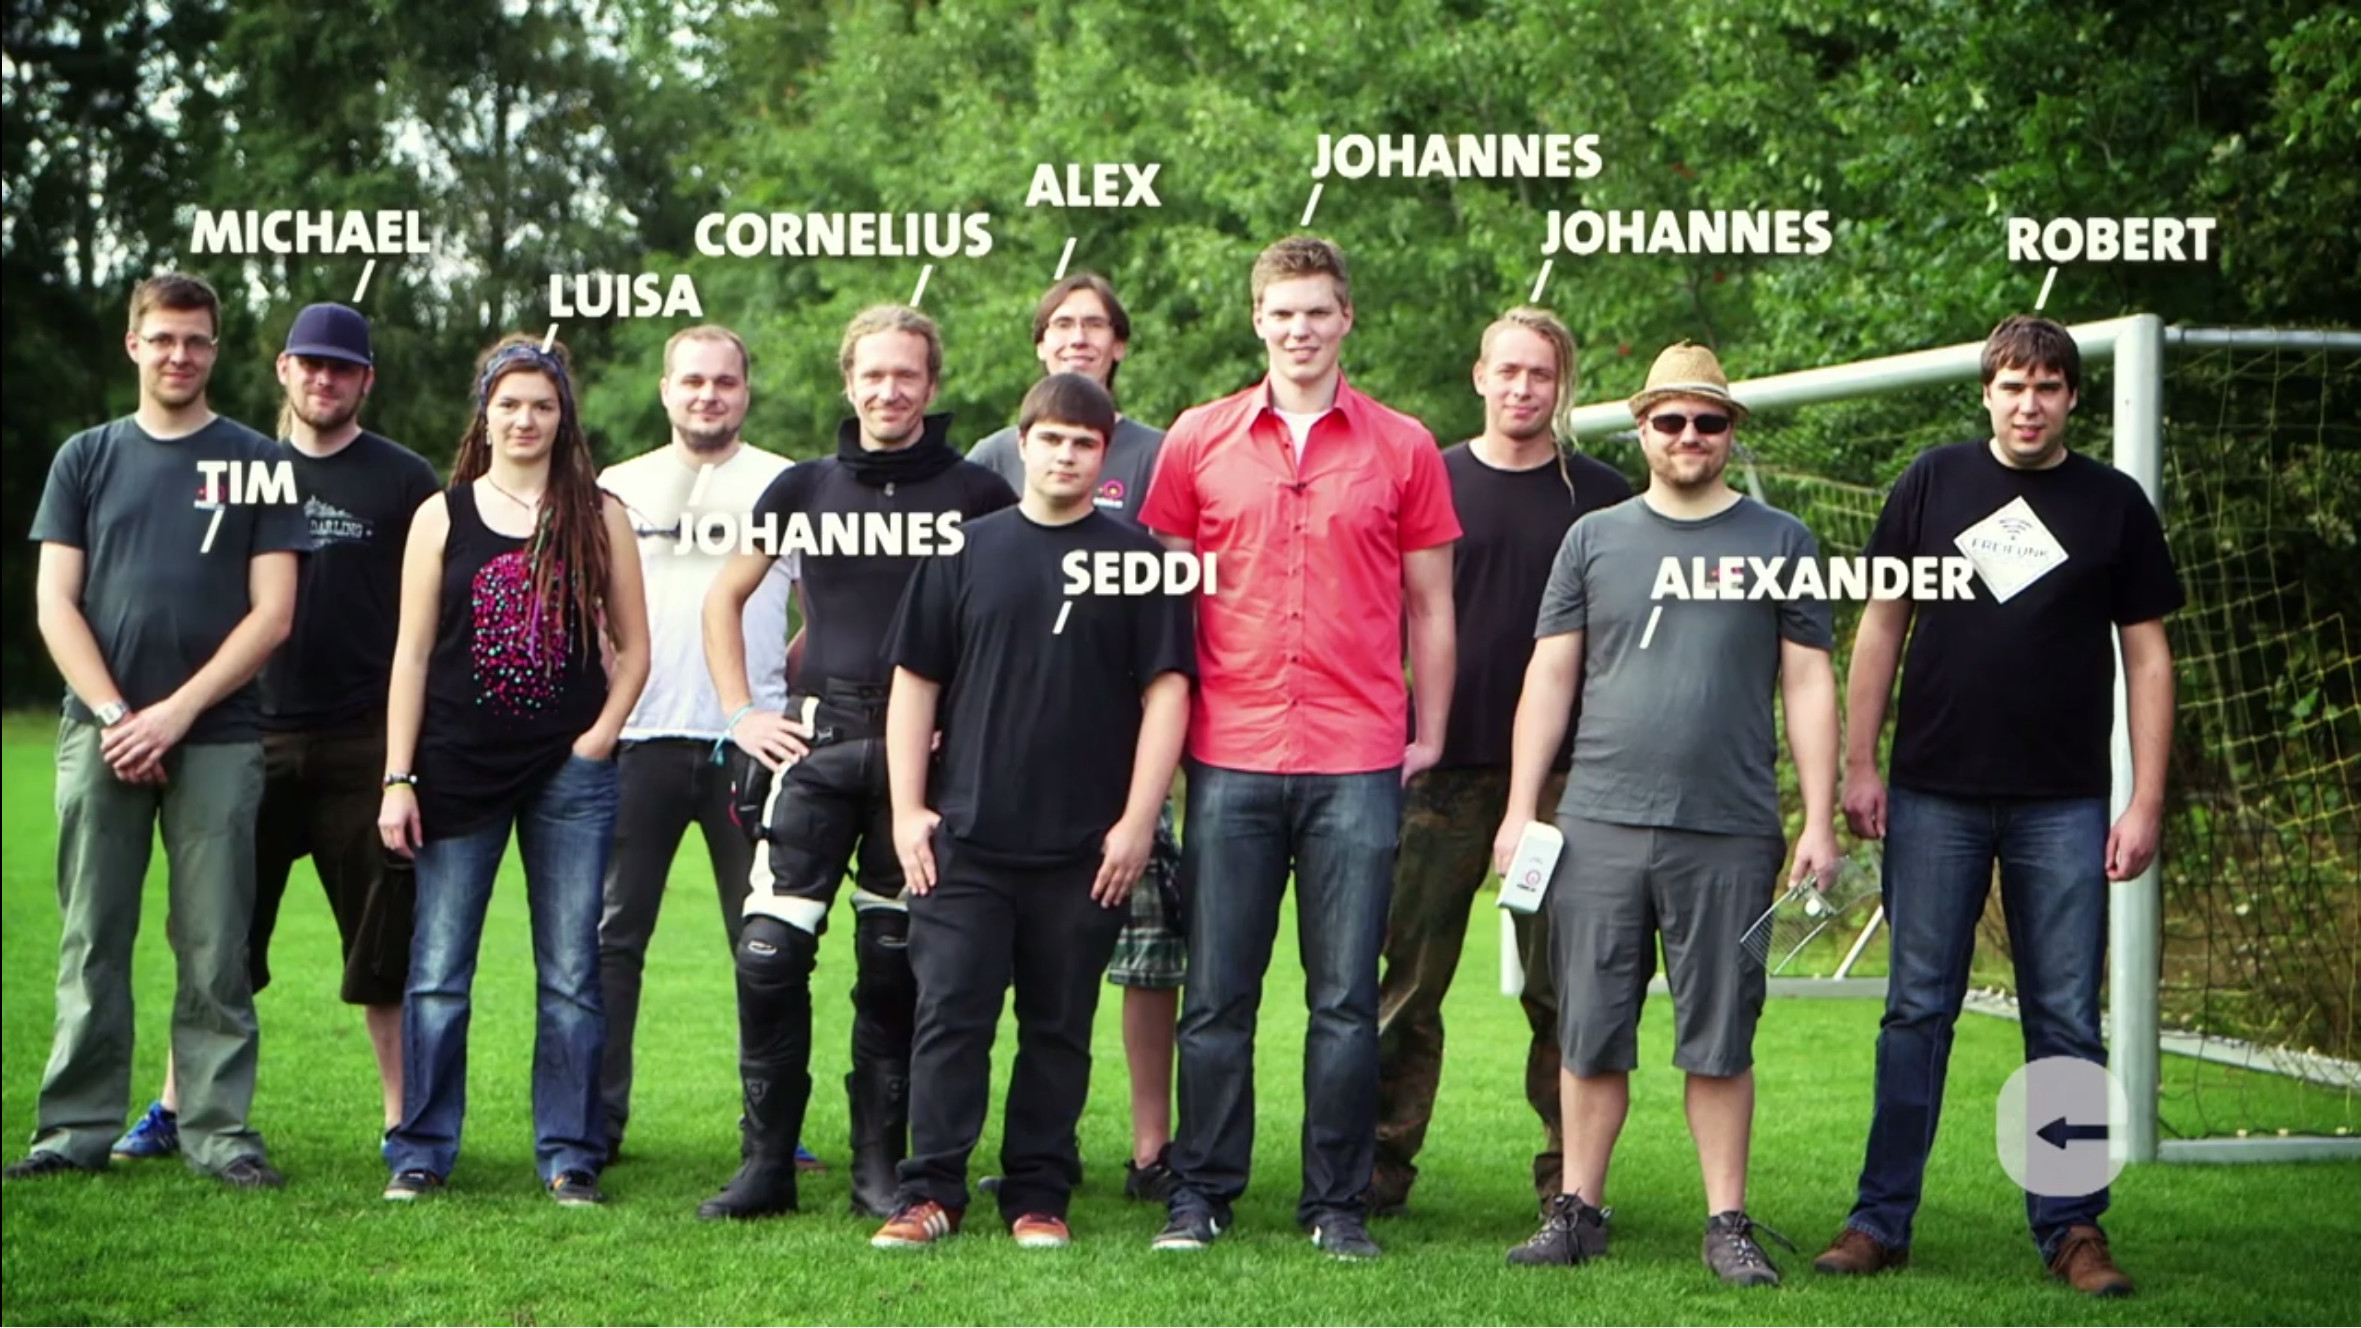
\includegraphics[width=\textwidth]{images/community.jpg}

\subsection{Snet - Entstehung & Verbreitung}

\begin{frame}
\frametitle{Verbreitung}
	\begin{itemize}
		\item Entstand 2011 als Verknüpfung von Heimnetzwerken für Gaming & Filesharing
		\item Mittlerweile Netzwerk aus mehr als 100.000 Nutzern
		\item Verteilung über Havanna:
			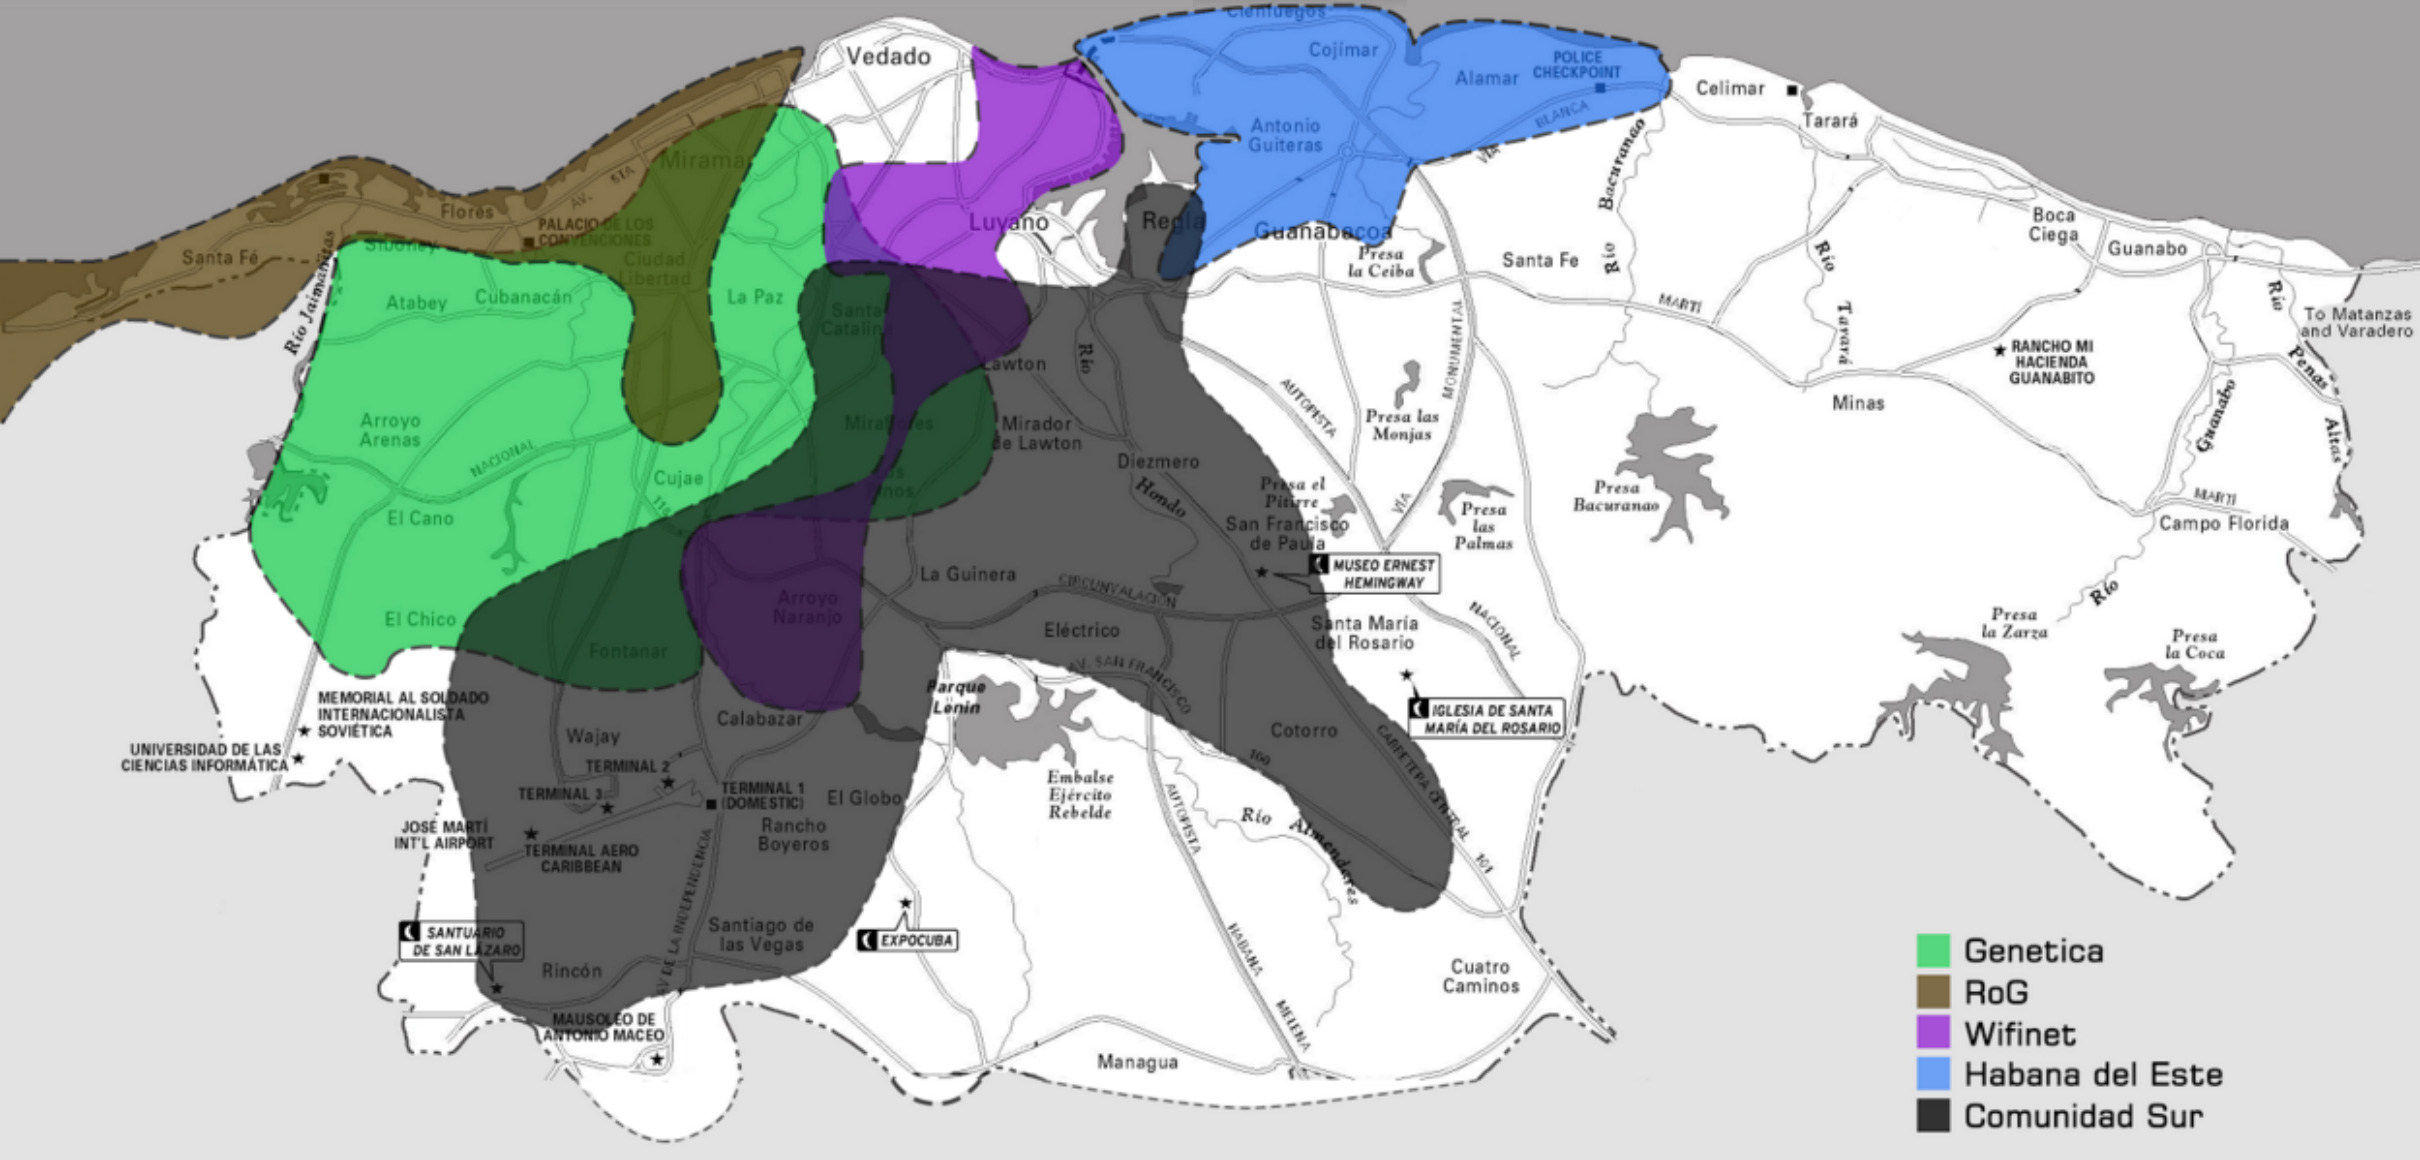
\includegraphics[width=\textwidth]{images/havanna_net.jpg}
	\end{itemize}
	
\end{frame}

\subsection{Technik & Hardware}

\begin{frame}
\frametitle{Schaut dann so aus:}
	\begin{itemize}
		\item Günstige Hardware erlaubt es Amatuer-Admins viele Knotenpunkte zu maintainen:
			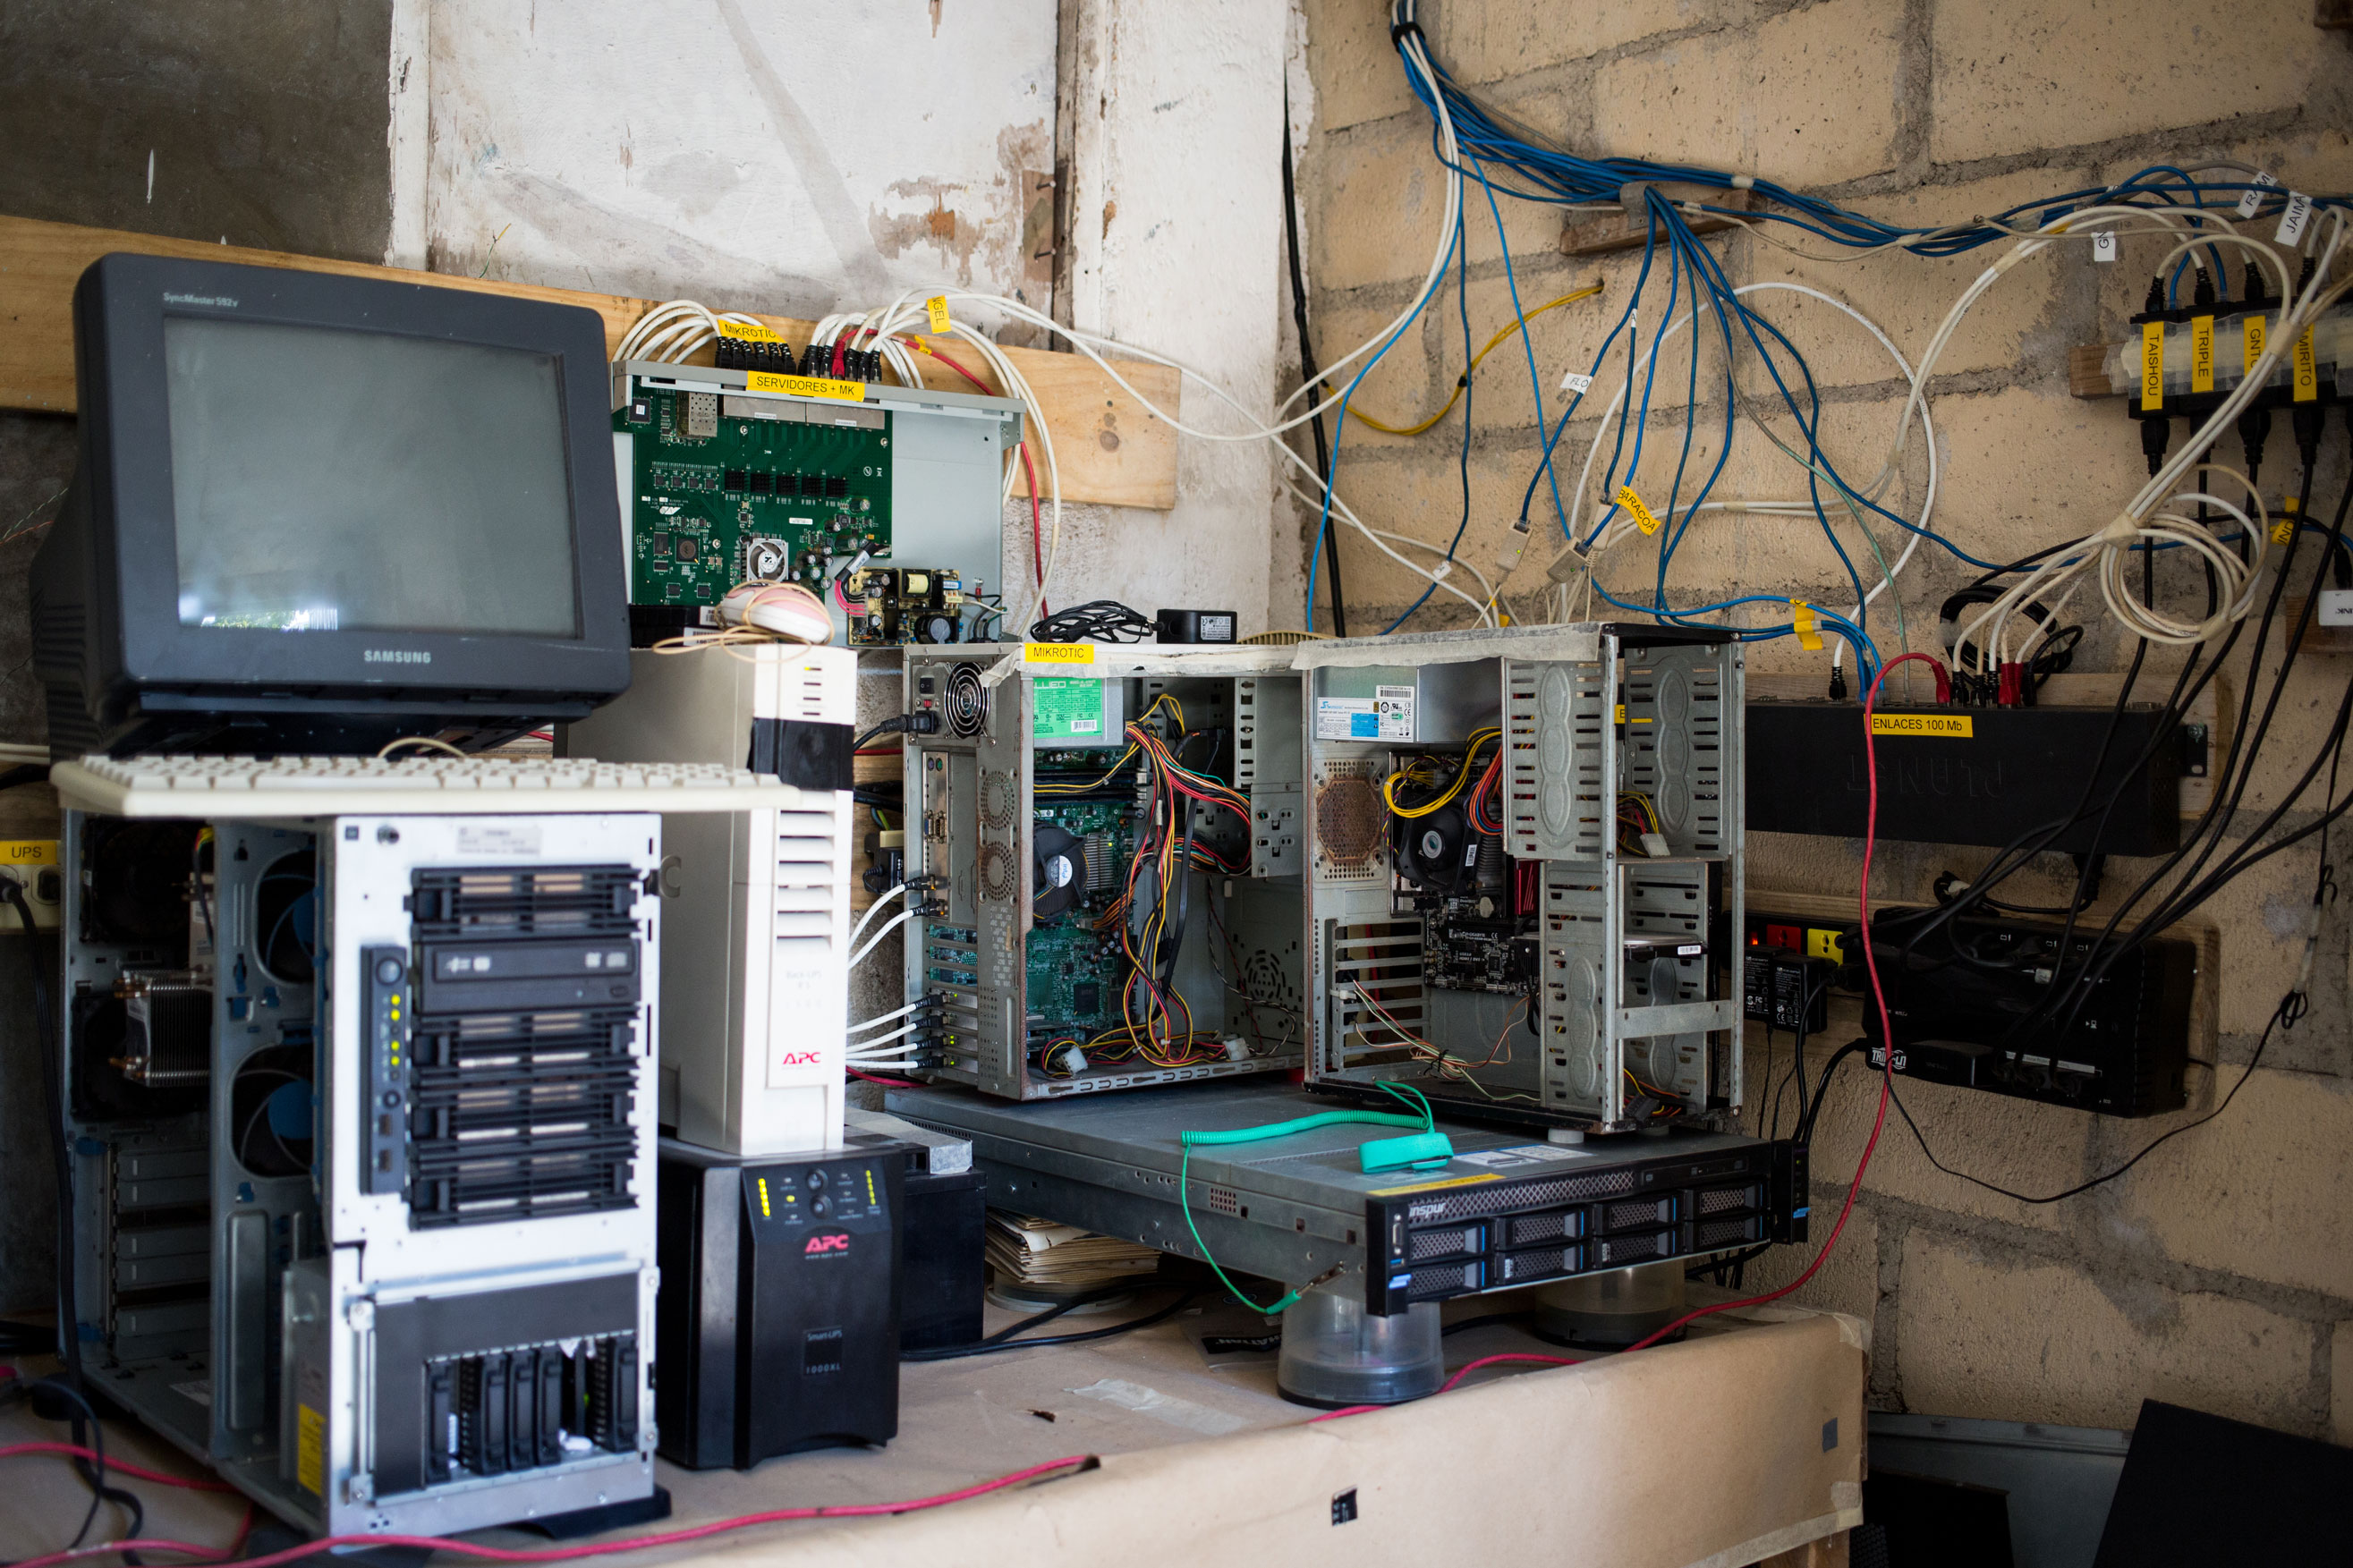
\includegraphics[width=\textwidth]{images/snet_pillar.jpg}
	\end{itemize}
\end{frame}